\section{系统功能与软件架构}
\label{sec:implementation}

本章把 IronBuddy 的软件层拆成总体架构、训练业务和交互维护三层：4.1
说明系统如何用多进程和共享状态把视觉、肌电、语音、前端与后台记录隔离
开；4.2 在该骨架上描述训练业务如何从单纯计数推进到兼顾目标肌激活与
代偿判断；4.3 说明语音状态机、调试控制台和本地数据库如何让系统在功能
持续扩展时仍可复测。

\begin{figure}[htbp]
    \centering
    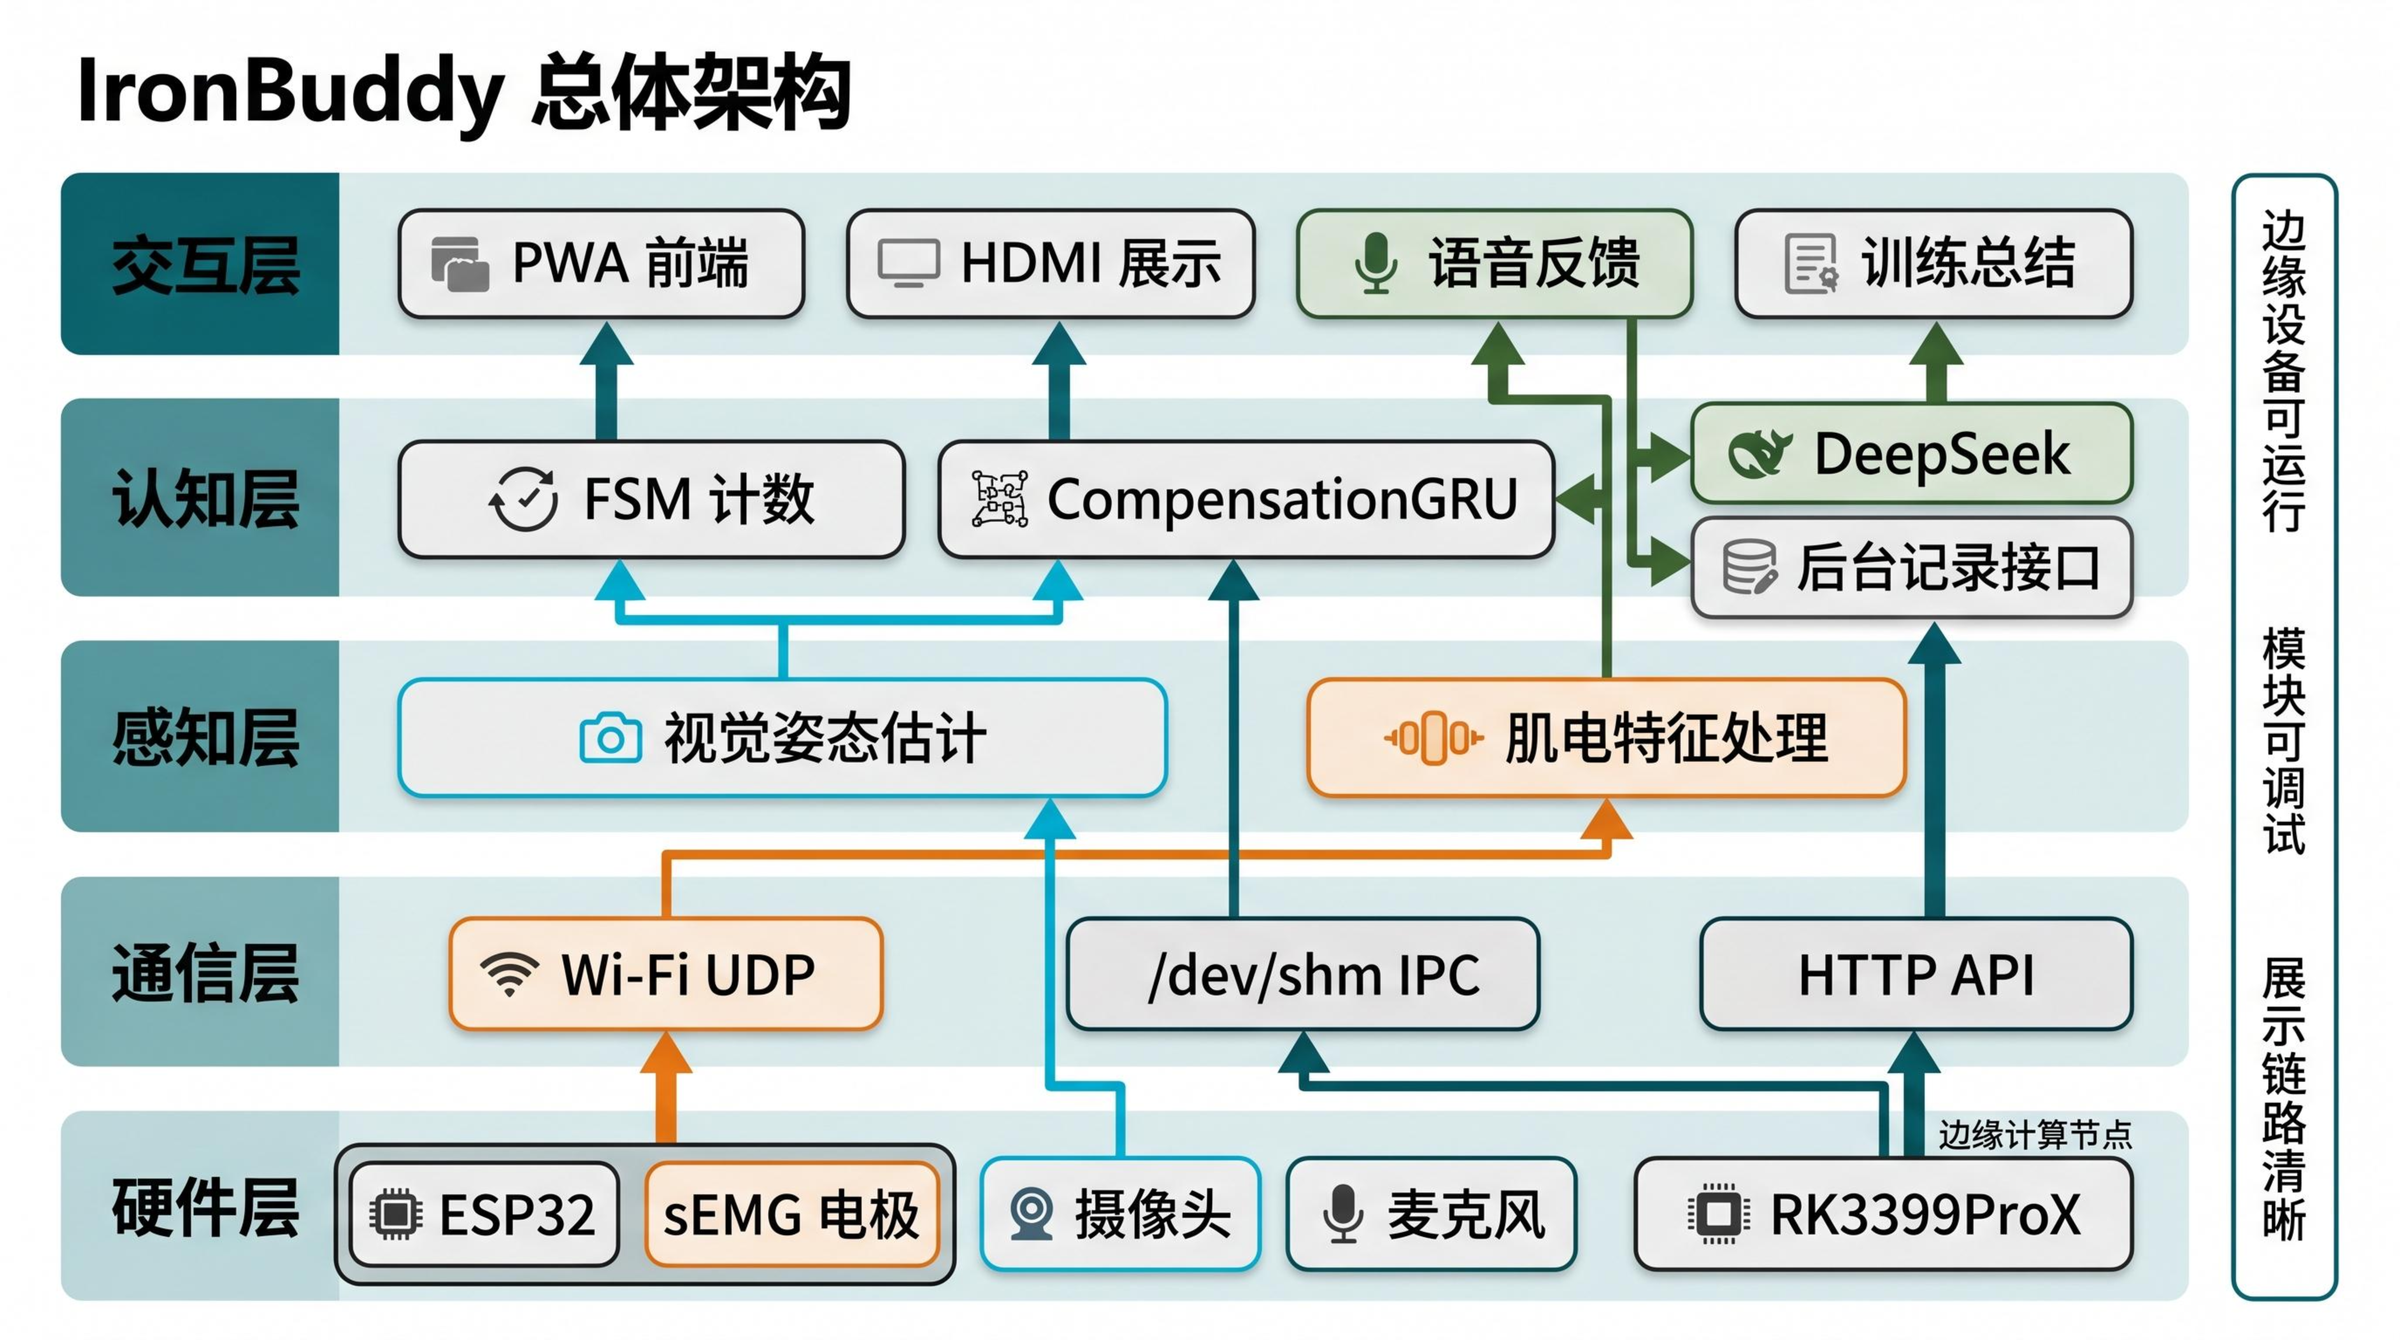
\includegraphics[width=0.92\textwidth]{figures/report/fig02.png}
    \caption{系统总体架构。}
    \label{fig:system-architecture}
\end{figure}

\subsection{软件总体：多进程与共享状态}

本节说明系统如何用多进程和共享状态把视觉、肌电、语音、前端与后台记录
隔离开。

\subsubsection{整体运行方式}

本项目的软件部分最终采用多进程结构。视觉、肌电、状态机、Web 服务和
语音逻辑分别运行，各自负责一类清楚的任务。早期把多种功能塞进同一主循环
时，摄像头、语音或前端任一环节卡住都会影响其他模块；拆分后，单个模块
异常更容易定位，也更适合现场调试。

\begin{table}[htbp]
\centering
\small
\begin{tabular}{@{}>{\raggedright\arraybackslash}p{0.23\textwidth}
                >{\raggedright\arraybackslash}p{0.31\textwidth}
                >{\raggedright\arraybackslash}p{0.34\textwidth}@{}}
\toprule
\textbf{模块} & \textbf{主要职责} & \textbf{典型输出} \\
\midrule
streamer\_app & Web 控制台、视频流、API 入口 & 页面状态、用户操作信号 \\
vision & 本地或云端姿态估计 & 关键点、关节角度、视觉模式 \\
main\_claw\_loop & FSM 计数、GRU 推理、训练状态 & 次数、动作质量、疲劳值 \\
udp\_emg\_server & 肌电 UDP 接收与特征处理 & 目标肌/代偿肌激活特征 \\
voice\_daemon & 语音唤醒、TTS、命令和对话 & 语音回复、动作切换、聊天状态 \\
\bottomrule
\end{tabular}
\caption{系统核心进程与职责划分}
\label{tab:processes}
\end{table}

这些进程之间主要通过 \code{/dev/shm} 下的 JSON 或文本文件交换状态。写入方
先写临时文件，再用 rename 替换正式文件，减少读到半截内容的概率。这个
方案不如消息队列完整，但它简单、透明、跨进程可见。调试时直接查看共享
状态文件，就能判断当前是视觉、肌电、FSM、语音还是前端出了问题。

\begin{figure}[htbp]
    \centering
    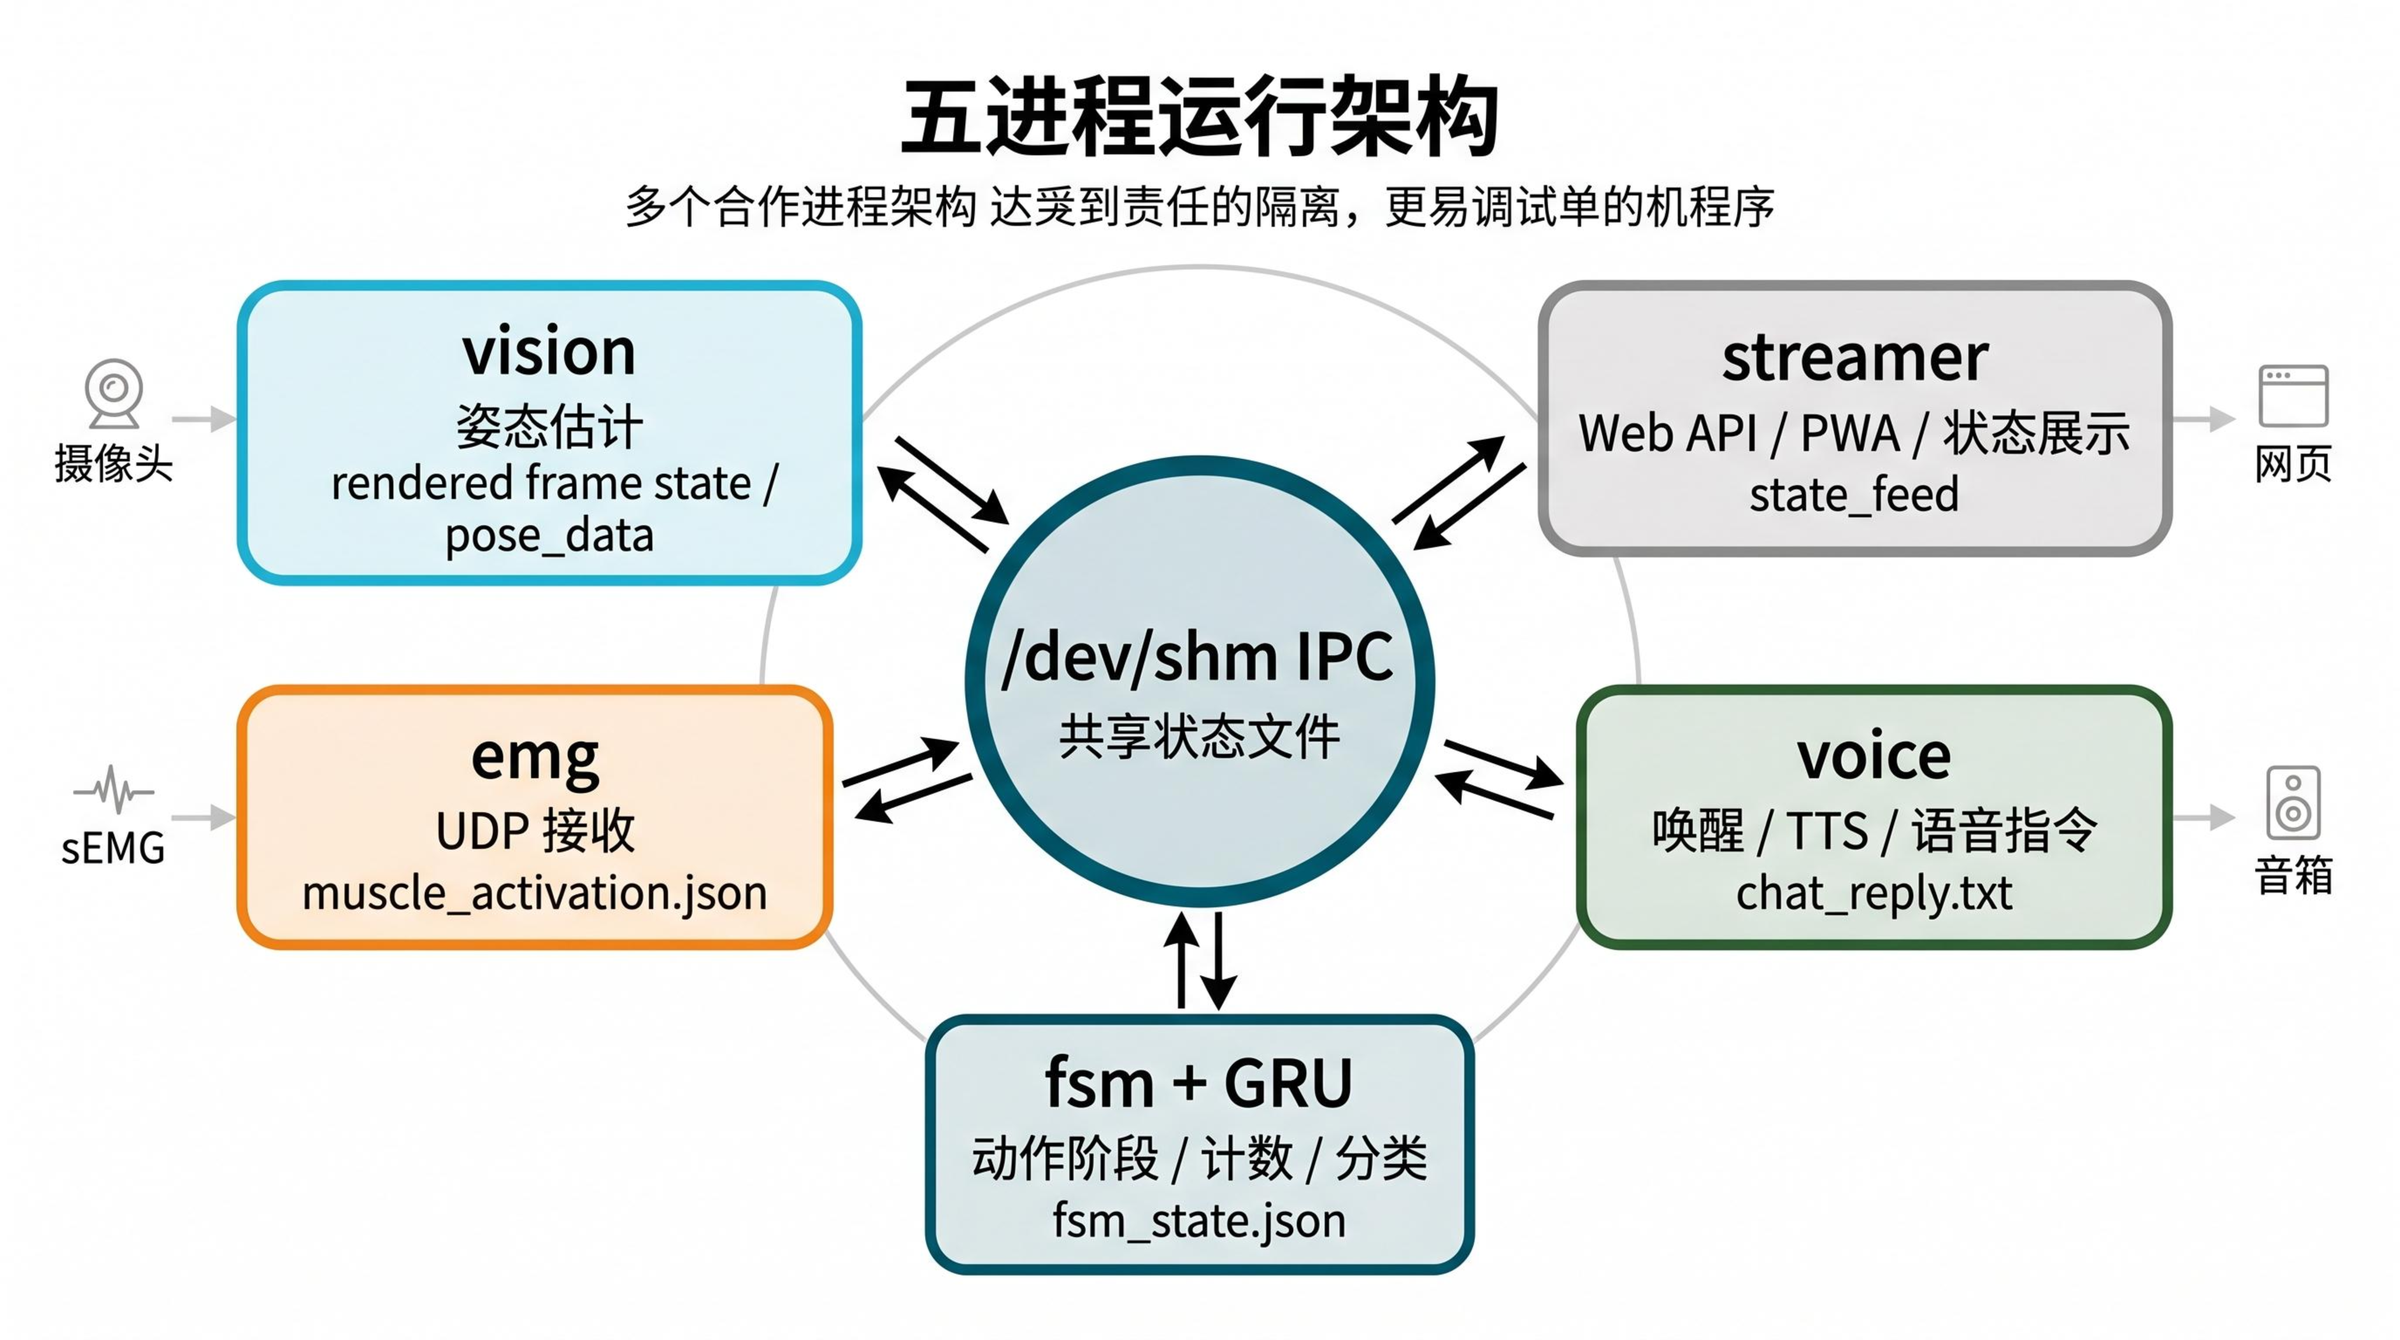
\includegraphics[width=0.9\textwidth]{figures/report/fig05.png}
    \caption{以共享状态文件为中心的进程协作方式。}
    \label{fig:ipc}
\end{figure}

\subsubsection{数据流与状态流}

一次训练中的数据流可以分为三条。第一条是视觉流：摄像头帧进入本地 NPU
或云端 RTMPose，输出关键点、关节角度和动作阶段参考。第二条是肌电流：
ESP32 将目标肌和代偿肌的采样特征通过 UDP 发送到板端，处理后写入肌肉
激活状态。第三条是交互流：用户通过语音或前端改变动作模式、疲劳上限和
视觉模式，系统再把这些意图写入共享状态文件。

这三条流最终在 FSM 和 GRU 处汇合。FSM 根据关节角度变化识别动作阶段和
完成次数，GRU 根据最近一段 7D 特征窗口判断动作质量，前端和语音再把这些
结果转化为可读反馈。这样的结构让每个模块都有明确输入和输出，也避免了
前端、语音和模型互相直接调用内部函数。

\begin{figure}[htbp]
    \centering
    \resizebox{0.96\textwidth}{!}{%
    \begin{tikzpicture}[
        node distance=0.65cm and 0.95cm,
        box/.style={draw, rounded corners=2pt, align=center, font=\small,
                    minimum height=0.72cm, minimum width=2.45cm},
        vision/.style={box, fill=cyan!9, draw=cyan!65!black},
        emg/.style={box, fill=orange!11, draw=orange!80!black},
        user/.style={box, fill=green!9, draw=green!55!black},
        state/.style={box, fill=teal!9, draw=teal!70!black, minimum width=3.0cm},
        judge/.style={box, fill=purple!7, draw=purple!55!black},
        outputbox/.style={box, fill=gray!8, draw=gray!65},
        arrow/.style={-{Latex[length=2mm]}, thick}
    ]
        \node[vision] (camera) {摄像头帧};
        \node[vision, right=of camera] (pose) {姿态估计\\关键点 / 角度};
        \node[emg, below=of camera] (esp) {ESP32 肌电};
        \node[emg, right=of esp] (emgfeat) {肌电特征\\RMS / MVC};
        \node[user, below=of esp] (intent) {用户意图\\语音 / 前端};
        \node[user, right=of intent] (mode) {训练参数\\动作 / 阈值};

        \node[state, right=1.25cm of pose, yshift=-0.72cm] (shm)
            {\code{/dev/shm}\\共享状态层};
        \node[judge, right=1.15cm of shm, yshift=0.58cm] (fsm)
            {FSM\\阶段 / 计数};
        \node[judge, right=1.15cm of shm, yshift=-0.58cm] (gru)
            {GRU\\质量判断};
        \node[outputbox, right=1.1cm of fsm] (feedback)
            {反馈输出\\语音 / 页面};
        \node[outputbox, right=1.1cm of gru] (record)
            {记录沉淀\\数据库 / 总结};

        \draw[arrow, cyan!70!black] (camera) -- (pose);
        \draw[arrow, orange!85!black] (esp) -- (emgfeat);
        \draw[arrow, green!60!black] (intent) -- (mode);
        \draw[arrow, cyan!70!black] (pose) -- (shm);
        \draw[arrow, orange!85!black] (emgfeat) -- (shm);
        \draw[arrow, green!60!black] (mode) -- (shm);
        \draw[arrow, teal!70!black] (shm) -- (fsm);
        \draw[arrow, teal!70!black] (shm) -- (gru);
        \draw[arrow, purple!60!black] (fsm) -- (feedback);
        \draw[arrow, purple!60!black] (gru) -- (feedback);
        \draw[arrow, purple!60!black] (fsm) -- (record);
        \draw[arrow, purple!60!black] (gru) -- (record);
    \end{tikzpicture}}
    \caption{训练过程中的数据流与状态流。}
    \label{fig:data-state-flow}
\end{figure}

\subsection{训练业务：从计数到结果导向}

在前面骨架基础上，本节描述训练业务如何从单纯计数转向兼顾目标肌激活与
代偿判断，并以一次完整流程为例说明各模块的协同。

\subsubsection{结果导向的训练方式}

本项目的一个重点是把训练记录从"做了几次"推进到"每次动作是否真正
练到了"。传统次数统计只能说明动作完成了多少个，却不能说明目标肌激活
是否充分，也不能区分标准发力和代偿发力。系统因此把次数放在基础层，把
目标肌激活、代偿肌比例和疲劳积分放在质量层。

具体落地参数上，视觉特征以 30 Hz 写入共享状态层，肌电特征以 100 Hz 由
ESP32 通过 UDP 上行后由板端聚合为 30 Hz 同步帧；GRU 推理在每一组动作
完成时触发一次，输入为最近 W=64 帧（约 2.1 s）的 7D 特征窗口，输出
标准 / 代偿 / 不标准三类。前端展示时，用户不仅看到完成次数，也能看到
疲劳积分、动作质量和代偿提示。疲劳积分是工程化训练负荷指标，综合完成
次数、动作质量与肌电激活趋势，用于提示本组训练是否接近上限；表面肌电
频域指标也常用于评估肌肉疲劳趋势 \cite{cifrek2009}，但本项目的疲劳
积分仅作为反馈和展示指标使用，不写为生理疲劳的严格度量。

\begin{algorithm}[htbp]
\caption{每帧 FSM 计数与 GRU 质量判断（以深蹲为例）}
\label{alg:fsm-gru}
\begin{algorithmic}[1]
\Require pose, emg from \texttt{/dev/shm}; thresholds $\theta_{\text{down}}, \theta_{\text{up}}$; window $W$
\State $f_t \gets$ Build7DFeature(pose, emg)
\Statex \quad \Comment{角度 / 角速度 / 角加速度 / 目标肌 RMS / 代偿肌 RMS / 对称性 / 相位}
\State Push $f_t$ into ring buffer of length $W$
\If{state $=$ UP $\land$ knee\_angle $< \theta_{\text{down}}$}
    \State state $\gets$ DOWN
\ElsIf{state $=$ DOWN $\land$ knee\_angle $> \theta_{\text{up}}$}
    \State state $\gets$ UP; \quad count $\mathrel{+}{=} 1$
    \State $y \gets$ \Call{GRU}{$f_{t-W+1:t}$}
    \Statex \quad \Comment{$y \in \{\text{good}, \text{compensated}, \text{bad}\}$}
    \State Append (count, $y$, fatigue) to \texttt{/dev/shm/rep\_event.json}
    \If{$y \neq \text{good}$} \State TriggerVoiceFeedback($y$) \EndIf
\EndIf
\end{algorithmic}
\end{algorithm}

算法 \ref{alg:fsm-gru} 也解释了为什么系统没有完全依赖神经网络计数：
计数本身是几何问题，用 FSM 更稳定；代偿识别才需要模型综合多个信号。
两者分工后，系统既能保留规则的可解释性，又能利用肌电补充纯视觉看不到
的信息。

\subsubsection{一次典型训练流程}

从用户视角看，一次训练可以自然串起上述模块。用户穿戴腰包、贴片和传感
线路后，通过语音或前端选择动作模式；视觉模块识别身体姿态，肌电模块上传
目标肌和代偿肌特征；FSM 根据动作阶段计数，GRU 在动作窗口内判断质量；
前端显示训练状态，语音在动作切换、MVC、疲劳接近上限或用户主动询问时
给出反馈。

这个流程的关键不是某个模块单独"很强"，而是各模块之间不要互相抢控制权。
前端可以写入疲劳上限，语音也可以写入；FSM 会触发总结，用户也可能正在
对话；TTS 播报时麦克风仍能听到声音。项目用共享状态文件、时间戳和状态机
把这些行为隔离开，使系统在功能越来越多时仍然保持可读和可调试。

\begin{figure}[htbp]
    \centering
    \resizebox{0.96\textwidth}{!}{%
    \begin{tikzpicture}[
        lane/.style={font=\bfseries\small, anchor=east},
        evt/.style={draw, rounded corners=2pt, fill=cyan!10, draw=cyan!65!black,
                    font=\scriptsize, inner sep=2.5pt, minimum height=0.55cm},
        evt2/.style={evt, fill=orange!12, draw=orange!75!black},
        evt3/.style={evt, fill=purple!9, draw=purple!60!black},
        evt4/.style={evt, fill=green!11, draw=green!55!black},
        evt5/.style={evt, fill=teal!11, draw=teal!70!black},
        ax/.style={->, gray!60, thick}
    ]
    % 五条泳道
    \foreach \y/\name in {0/用户, -1/视觉, -2/肌电, -3/FSM/GRU, -4/反馈}
        \node[lane] at (-0.2,\y) {\name};
    % 时间轴
    \foreach \y in {0,-1,-2,-3,-4}
        \draw[ax] (0,\y) -- (15.5,\y);
    \node[font=\scriptsize, anchor=west] at (15.5,-2) {$t$};

    % 事件块 (时间, lane, 类型, 文字)
    \node[evt5] at (1.2,0) {唤醒"教练"};
    \node[evt5] at (3.2,0) {选择动作};
    \node[evt4] at (5.7,0) {开始第 1 组};
    \node[evt4] at (12.6,0) {主动询问};

    \node[evt] at (5.7,-1) {骨架@30Hz};
    \node[evt] at (8.5,-1) {阶段=DOWN};
    \node[evt] at (10.2,-1) {阶段=UP};
    \node[evt] at (13.5,-1) {骨架@30Hz};

    \node[evt2] at (5.7,-2) {RMS@100Hz};
    \node[evt2] at (8.5,-2) {激活峰值};
    \node[evt2] at (10.2,-2) {代偿信号};
    \node[evt2] at (13.5,-2) {RMS@100Hz};

    \node[evt3] at (8.5,-3) {计数+1};
    \node[evt3] at (10.4,-3) {GRU=代偿};
    \node[evt3] at (12.0,-3) {疲劳累积};

    \node[evt5] at (3.2,-4) {TTS 引导};
    \node[evt5] at (10.6,-4) {语音提示};
    \node[evt5] at (12.8,-4) {DeepSeek 答复};

    % 关键依赖箭头
    \draw[->, dashed, gray!70] (8.5,-1) -- (8.5,-2.7);
    \draw[->, dashed, gray!70] (8.5,-2) -- (8.5,-2.85);
    \draw[->, dashed, gray!70] (10.2,-1) -- (10.4,-2.7);
    \draw[->, dashed, gray!70] (10.2,-2) -- (10.4,-2.85);
    \draw[->, dashed, gray!70] (10.4,-3) -- (10.6,-3.7);
    \draw[->, dashed, gray!70] (12.6,0) -- (12.8,-3.7);
    \end{tikzpicture}}
    \caption{一次完整训练的多模块时序示意。}
    \label{fig:training-timeline}
\end{figure}

\subsection{交互与维护：语音、调试控制台与数据库}

交互层与维护层共享同一套状态文件。本节说明语音状态机、调试控制台和
数据库如何让系统在功能扩展时仍可复测。

\subsubsection{语音交互与冲突仲裁}

语音模块面向的是运动中的真实操作场景。用户可能正在拿哑铃、做深蹲或佩戴
贴片，此时触屏并不自然。系统因此把动作切换、疲劳上限调整、MVC 引导、
训练总结和简单问答都接入语音链路，让前端更多承担展示和调试入口。

语音链路的难点在于冲突仲裁。用户主动唤醒、系统自动总结和 TTS 播报可能
同时发生；如果没有状态管理，系统播报的声音还可能被麦克风录回去。后期
重构把语音逻辑整理为 LISTEN、DIALOG、BUSY 三个状态。LISTEN 等待唤醒，
DIALOG 处理用户一轮指令或问答，BUSY 处理 TTS、MVC 流程和自动总结。BUSY
期间暂停录音，降低自录和串音风险。

\begin{figure}[htbp]
    \centering
    \resizebox{0.82\textwidth}{!}{%
    \begin{tikzpicture}[
        state/.style={draw, rounded corners=3pt, align=center, minimum width=3.0cm,
                      minimum height=1.0cm, font=\small},
        listen/.style={state, fill=teal!12, draw=teal!70!black},
        dialog/.style={state, fill=green!10, draw=green!55!black},
        busy/.style={state, fill=orange!14, draw=orange!80!black},
        note/.style={draw, rounded corners=2pt, align=center, fill=red!5,
                     draw=red!45!black, font=\small, minimum width=3.8cm},
        arrow/.style={-{Latex[length=2mm]}, thick}
    ]
        \node[listen] (listen) {LISTEN\\等待唤醒 / 监听"教练"};
        \node[dialog, right=3.4cm of listen] (dialog) {DIALOG\\识别指令 / 调用对话或工具};
        \node[busy, below=2.1cm of dialog] (busy) {BUSY\\TTS 播报 / MVC 流程 / 自动总结};
        \node[note, left=2.1cm of busy] (note) {BUSY 期间暂停录音\\减少 TTS 被再次录入};

        \draw[arrow, teal!70!black] (listen) -- node[above, font=\small]{唤醒词或语音指令} (dialog);
        \draw[arrow, green!55!black] (dialog) -- node[right, font=\small]{生成回复或触发流程} (busy);
        \draw[arrow, orange!80!black] (busy.west) -- ++(-1.0,0) |- node[pos=0.24, left, font=\small]{播报完成 / 流程结束} (listen.south);
        \draw[arrow, gray!70!black] (dialog.north) to[bend left=30]
            node[above, font=\small]{没听清或超时归位} (listen.north);
        \draw[arrow, red!55!black] (note) -- (busy);
    \end{tikzpicture}}
    \caption{语音模块的三状态模型。}
    \label{fig:voice-state}
\end{figure}

\subsubsection{统一状态观察与端到端调试控制台}

系统进入后期后，主要困难不再是单个功能能否跑通，而是如何在一个已经成型
的端到端项目中继续升级。视觉、肌电、FSM、语音、LLM、数据库和 Web 前端
之间存在大量状态依赖；如果只凭直觉修改代码，很容易修好一个局部，又在
另一条链路上引入新问题。因此，本项目搭建了一套面向多模块协同维护的
端到端调试控制台，把状态观察、问题定位、修改建议和复测记录组织成固定流程。

这套工作台的核心不是增加一个独立页面，而是建立可被人和工具共同读取的
调试表征。系统把关键运行状态、知识库命中、云端记忆、数据库记录、代码
结构关系和测试步骤整理到统一入口中。这样在添加新功能或修复旧问题时，
可以先确认当前现象，再定位涉及的模块和状态文件，随后根据复测记录检查
修改是否真的改善了端到端结果。

这种设计让外部协作者不必从零理解项目，也能围绕真实运行状态、历史记录和
代码结构提出修改建议，再根据复测结果决定是否保留。对于包含多进程、
传感器、语音和前端的系统来说，这种结果导向的调试方式比盲目重构更稳，
也更适合后续长期维护。

\begin{figure}[htbp]
    \centering
    \resizebox{0.92\textwidth}{!}{%
    \begin{tikzpicture}[
        center/.style={draw, rounded corners=4pt, align=center,
                       fill=teal!13, draw=teal!70!black, font=\bfseries\small,
                       minimum width=3.4cm, minimum height=1.1cm},
        panel/.style={draw, rounded corners=3pt, align=center, font=\small,
                      minimum width=3.0cm, minimum height=0.95cm},
        p1/.style={panel, fill=cyan!10, draw=cyan!65!black},
        p2/.style={panel, fill=orange!11, draw=orange!75!black},
        p3/.style={panel, fill=purple!8, draw=purple!60!black},
        p4/.style={panel, fill=green!10, draw=green!55!black},
        p5/.style={panel, fill=red!7, draw=red!55!black},
        arrow/.style={-{Latex[length=2mm]}, thick, gray!70}
    ]
        \node[center] (hub) at (0,0) {端到端调试控制台\\\scriptsize ironbuddy\_operator\_console};
        \node[p1] (a) at (-5.5, 1.6) {运行状态\\\scriptsize 5 个进程心跳};
        \node[p2] (b) at (-5.5,-1.6) {传感验证\\\scriptsize 视频 / EMG 波形};
        \node[p3] (c) at ( 0, 2.6) {知识库命中\\\scriptsize RAG-lite 检索};
        \node[p4] (d) at ( 5.5, 1.6) {数据库视图\\\scriptsize 5 张表 + 记录};
        \node[p5] (e) at ( 5.5,-1.6) {代码结构关系\\\scriptsize 模块依赖图};
        \node[panel, fill=gray!8, draw=gray!60] (f) at ( 0,-2.6) {复测记录\\\scriptsize 手测脚本 + 截图};

        \draw[arrow] (a) -- (hub); \draw[arrow] (b) -- (hub);
        \draw[arrow] (c) -- (hub); \draw[arrow] (d) -- (hub);
        \draw[arrow] (e) -- (hub); \draw[arrow] (f) -- (hub);
    \end{tikzpicture}}
    \caption{端到端调试控制台的六个观察面板。}
    \label{fig:debug-console}
\end{figure}

\subsubsection{训练记录与长期接口}

训练系统如果只看当前一组动作，很难在后续迭代中复盘问题。本项目因此
保留了本地数据库和训练记录接口：每次训练产生的动作、疲劳、对话和总结
都可以沉淀为后续分析材料。数据库不仅保存记录，也为后续模型迭代、训练
周报、偏好学习和个性化建议留下接口。

\begin{figure}[htbp]
    \centering
    \begin{subfigure}[t]{0.46\textwidth}
        \centering
        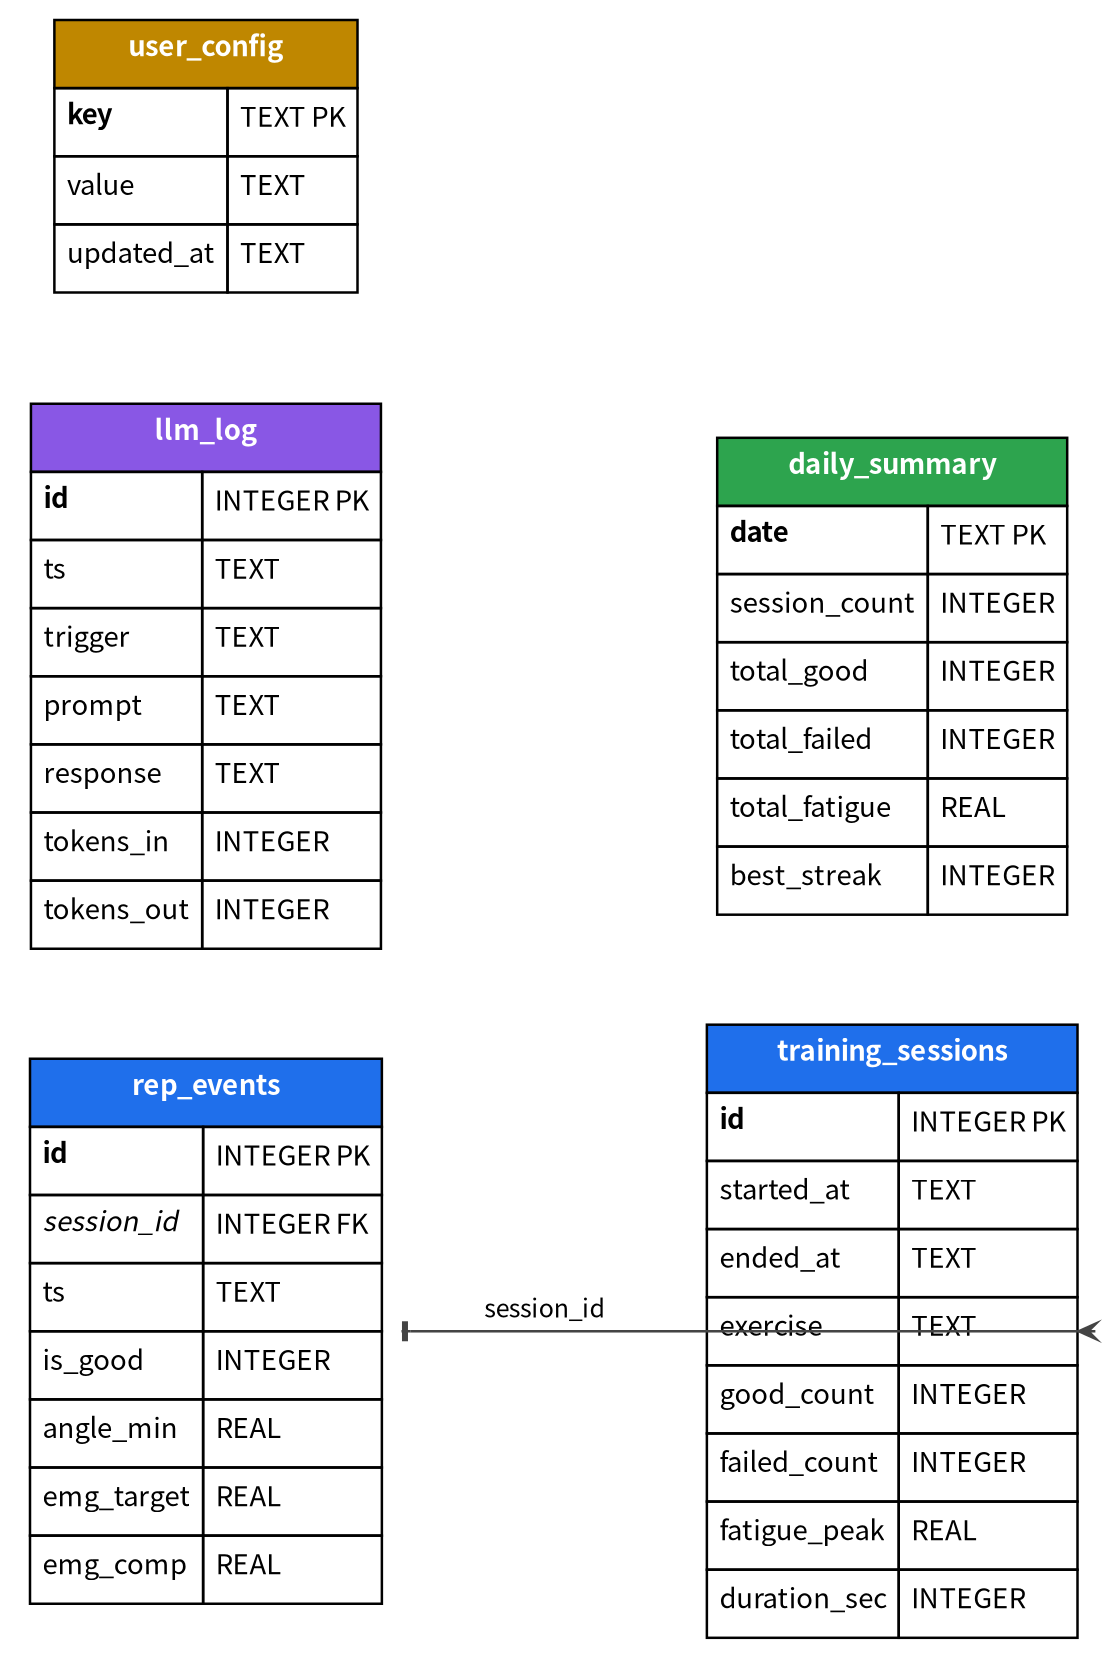
\includegraphics[width=\linewidth]{figures/report/fig09a-er.png}
        \caption{表关系（ER）视图}\label{fig:db-er}
    \end{subfigure}\hfill
    \begin{subfigure}[t]{0.50\textwidth}
        \centering
        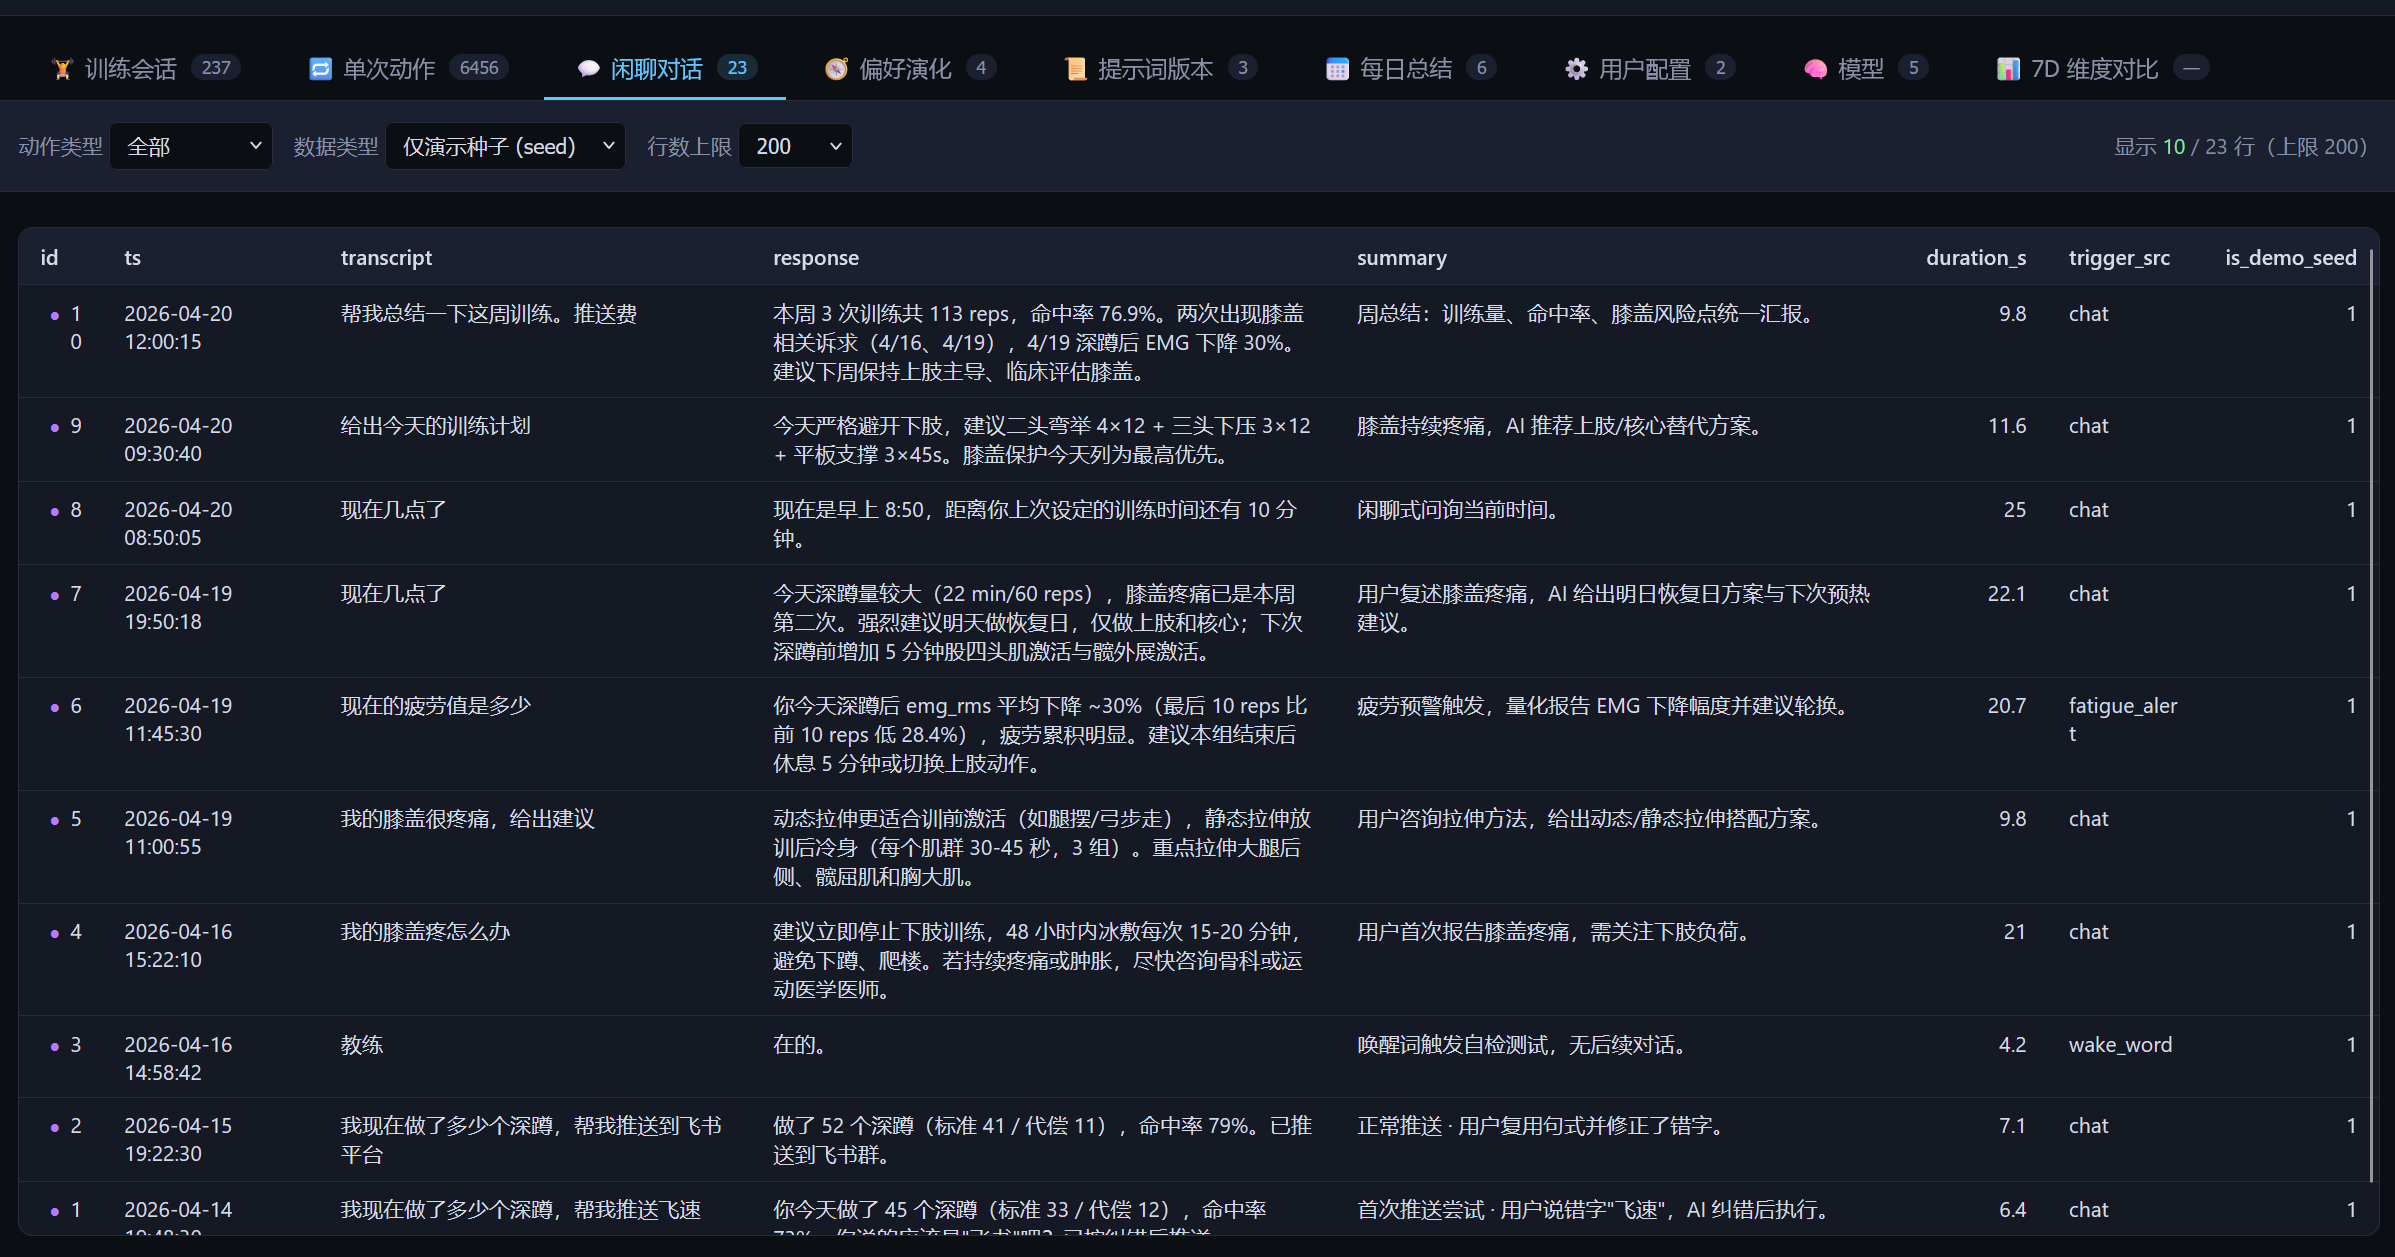
\includegraphics[width=\linewidth]{figures/report/fig09b-record.png}
        \caption{对话记录子表示例}\label{fig:db-record}
    \end{subfigure}
    \caption{本地训练记录数据库的 ER 视图与记录示例（5 张表：\texttt{training\_sessions} 训练会话、\texttt{rep\_events} 单次动作、\texttt{llm\_log} 对话日志、\texttt{daily\_summary} 每日总结、\texttt{user\_config} 用户配置）。}
    \label{fig:database}
\end{figure}

数据库记录为长期个性化分析预留了数据基础，能够把训练过程、用户问题、
总结文本和偏好变化沉淀下来。随着真实训练数据和复测流程继续积累，这些
记录可以进一步支持用户偏好建模、周期性训练总结和更稳定的个性化建议。

\subsection*{本章小结}
\addcontentsline{toc}{subsection}{本章小结}

本章把 IronBuddy 的软件层拆成总体架构、训练业务和交互维护三层。多进程
与共享状态保证了模块边界，结果导向的训练业务把计数推进到了质量判断，
语音状态机、调试控制台和本地数据库则让系统在功能持续扩展时仍能保持
可读、可复测。
